\documentclass[
    UTF8,
    12pt,
    oneside,
    a4paper
]{ctexart}

\usepackage{geometry}
\usepackage{graphicx}
\usepackage{float}

\setmainfont{Times New Roman}
\geometry{
    a4paper,
    left=2cm,
    right=2cm,
    top=3cm,
    bottom=3cm
}
\pagestyle{plain}

\title{EL 项目中期文档}
\date{\today}
\author{撰写人:\wo}

\def\PUBLICVERSION{}

\ifdefined\PUBLICVERSION
    \newcommand\wo{\textsf{pilgrimlyieu}}
\newcommand\rr{\textsf{KashingLiking}}
\newcommand\vi{\textsf{t0mo0n}}
\newcommand\tv{\textsf{EnndWang}}

\else
    \input{private.tex}
\fi

\begin{document}

\maketitle

\section{作品目标}

\subsection{背景介绍}

科技发展日新月异,各种突破人们想象力的产品层出不穷。同时中华传统文化博大精深,历史悠久。尤其是诗词,更是当中的瑰宝,是文艺创作中的重要组成部分。

然而科学技术的高歌猛进并没有在同时带动中华优秀传统文化方面的高速发展。在这种情况下,我们小组希望借助现代科技手段,结合我们现有的知识储备,探索科技在文化领域的创新应用,从而推动文化的发展与传播,使得传统文化能够更好地传承和发扬。

而文字始终是文化传播的重要载体,也是文艺宣传最为关键的一环。诗词又是中华文化的精髓,是文艺作品中不可多得的精华。因此我们小组决定以文字创作工具为切入点,设计一款\emph{能够帮助用户方便地将诗词融入自己文艺作品中的\textbf{创作工具}},在此基础上\emph{使用户对我国的诗词文化有更深入的了解},同时期许辅以大模型、OCR 等前沿技术,\emph{辅助用户进行文化创作}。

同时我们还构想在此工具的基础上衍生出一个创作平台,使得用户可以在此平台上分享自己的作品,与他人交流,并获得他人的反馈等,从而更进一步,从一个更高的维度促进文化的交流与传播。但是出于时间紧迫,因此我们还是将重心放在了项目的核心,也就是创作工具的设计与实现上。并期许在未来的时间里,能够进一步完善这个目标。

\subsection{作品简介}

由于我们均没有任何开发经验,我们决定采用可能相对容易上手的 Web 应用的形式作为我们的作品形式。除了这个最为重要的原因外,我们还有以下几个考虑,因此最终还是选择了 Web 应用:

\begin{enumerate}
    \item Web 应用可以跨平台使用,用户可以在任何设备上使用我们的应用,而不需要担心设备的兼容性问题。
    \item Web 应用的开发相对容易上手,我们可以利用现有的工具和框架,快速地搭建起我们的应用。
    \item Web 应用的形式更贴合我们的目标,用户在进行文艺的文字创作过程中,势必要查阅相关资料,从而会频繁地使用浏览器,使用 Web 应用可以降低切换应用造成的割裂感。
    \item Web 应用与我们更进一步的社区构想也更加契合,不需要安装任何软件,所有人都可以进行访问并参与建设,有利于活跃社区氛围,促进文化交流与传播。
\end{enumerate}

\begin{figure}[H]
    \centering
    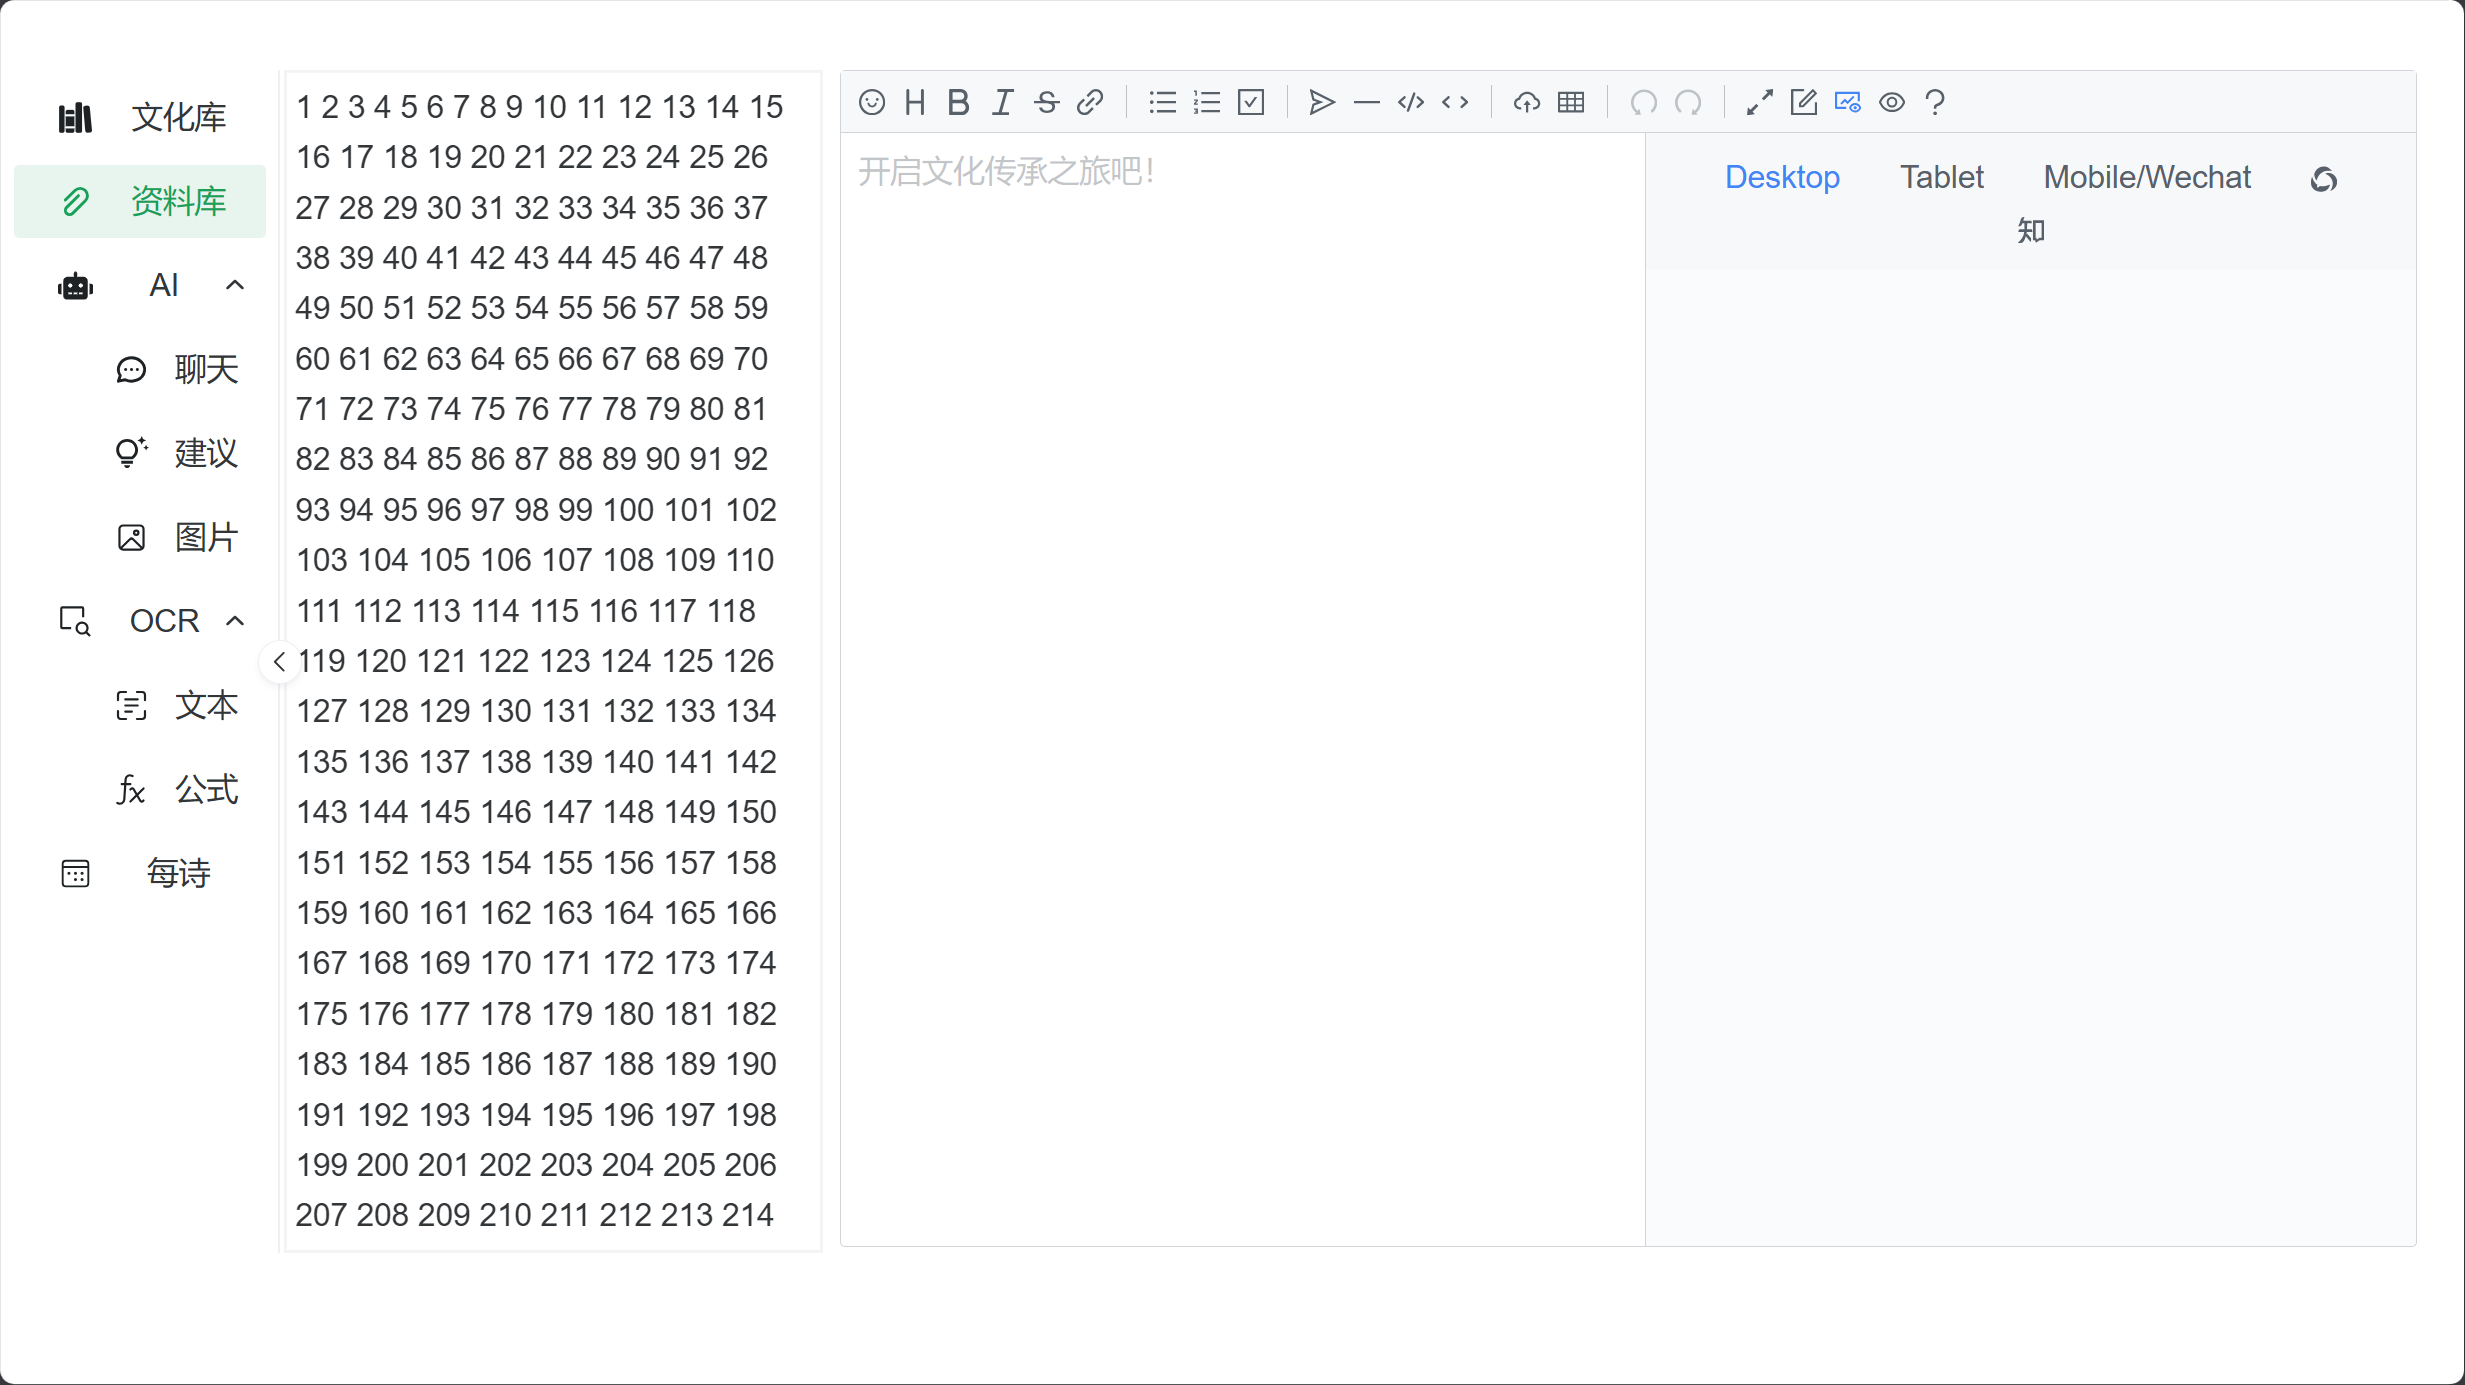
\includegraphics[scale=0.18]{../../stuff/img/05-10_process.png}
\end{figure}

如图所示大致是我们的基本框架,同时也是目前我们的项目完成情况。左侧是仿照 VS~Code 的插件栏,用户可以方便地选择自己想要使用的辅助创作的手段,而中间及右侧则是用户创作区域,即一个 Markdown 编辑器。

使用 Markdown 编辑器而非寻常的富文本编辑器主要基于以下几点考虑:

\begin{enumerate}
    \item Markdown 语法简单易懂,用户可以快速上手。
    \item Markdown 将内容与样式分离,用户可以专注于内容的创作,而不用过多关心样式。这也避免了用户舍本逐末,过度关注样式方面的细节,从而影响创作的效率。
    \item 该 Markdown 编辑器提供了 WYSIWYG (What You See Is What You Get, 所见即所得) 的功能,即使是不熟悉 Markdown 语法的用户也可以方便地按富文本编辑器的方式进行创作。
    \item 该 Markdown 编辑器提供了额外的「复制到知乎」「复制到公众号」等分享功能,可以进一步扩大文艺作品的传播范围,有利于进行文化交流与宣传。
\end{enumerate}

左侧的功能栏则是我们项目的特色所在,下面对我们目前的计划进行简单的介绍:

\begin{enumerate}
    \item \textbf{文化库}:这也是我们项目的核心功能,我们预计在其中按标签对诗词进行分类,同时按受欢迎程度进行排序,使用户可以根据自己的创作需求,方便地查找到自己想要的诗词。
    \item \textbf{资料库}:由于大众并没有接受过相对完善的信息教育,许多人的信息检索能力不强,因此在这里我们计划将一些常见的资料库进行汇总整理,也方便用户进行查阅。
    \item \textbf{AI}:我们期望使用最近热火朝天的大模型技术,使之既能与用户进行交流,又能为用户创作提供指导与建议,还能按照用户需求进行配图等。
    \item \textbf{OCR}:为了方便用户对自己的纸质作品进行电子化,以及一些用户可能对一些古籍进行研究,抑或是有些用户可能有引用却无法复制的需求,我们也希望提供 OCR 功能,以满足这些用户的需求。
    \item \textbf{每诗}:我们不仅想让诗词融入到用户的文艺作品中,还希望能够成为用户自身的一部分,因此我们希望提供随机显示诗词的功能,展示诗词背后的故事,从而使用户在创作的同时也能够进行文化的学习。
\end{enumerate}

\section{人员分工}

我们组本由四名成员(组长加粗)组成,分别是:

\begin{itemize}
    \item \textbf{\wo}
    \item \vi
    \item \rr
    \item \tv
\end{itemize}

后{\tv}因个人原因退出了项目,因此我们组目前分工如下:

\begin{itemize}
    \item \textbf{\wo}
        \begin{enumerate}
            \item 项目统筹规划
            \item 撰写小组组会记录、个人纪录、项目中期与最终报告、各类文档等
            \item 答辩 PPT 制作
            \item 资料搜寻与汇总
            \item 项目流程控制
            \item 项目代码审查
            \item 同时参与前后端开发(当前是前端为主)
        \end{enumerate}
    \item \vi
        \begin{enumerate}
            \item 前后端知识学习
            \item 后端开发
            \item 答辩 PPT 制作
        \end{enumerate}
    \item \rr
        \begin{enumerate}
            \item 前后端知识学习
            \item 后端开发
        \end{enumerate}
\end{itemize}

\section{当前进度}

我们计划采用 Vue3 作为前端框架,使用 NaiveUI 作为组件库,Flask 作为后端框架。

我们也借助了一些现代的工具,如在组长的指导下,每个组员都使用了 VS Code 进行开发,Black 等格式化工具进行代码格式化,以及 Copilot 进行辅助代码编写等。

同时我们使用 Git 进行版本管理,使用 GitHub 进行代码托管。每个组员在各自的分支进行开发,并在阶段性工作完成后提交 Pull Request,由组长进行代码审查,无误后最终合并到主分支。

目前有的分支:

\begin{enumerate}
    \item \textbf{\texttt{main}}:主分支,用于发布版本
    \item \texttt{doc}:\wo 用于文档编写的分支
    \item \texttt{feph}:\wo 开发的分支
    \item \texttt{maoyr1}:\vi 开发的分支
    \item \texttt{KashingLi}:\rr 开发的分支
    \item \texttt{enndwang}:前组员\tv 开发的分支
    \item \texttt{init}:项目初始化分支,已合并,故废弃
\end{enumerate}

下面便是目前的 Git commits 记录:

\begin{figure}[H]
    \centering
    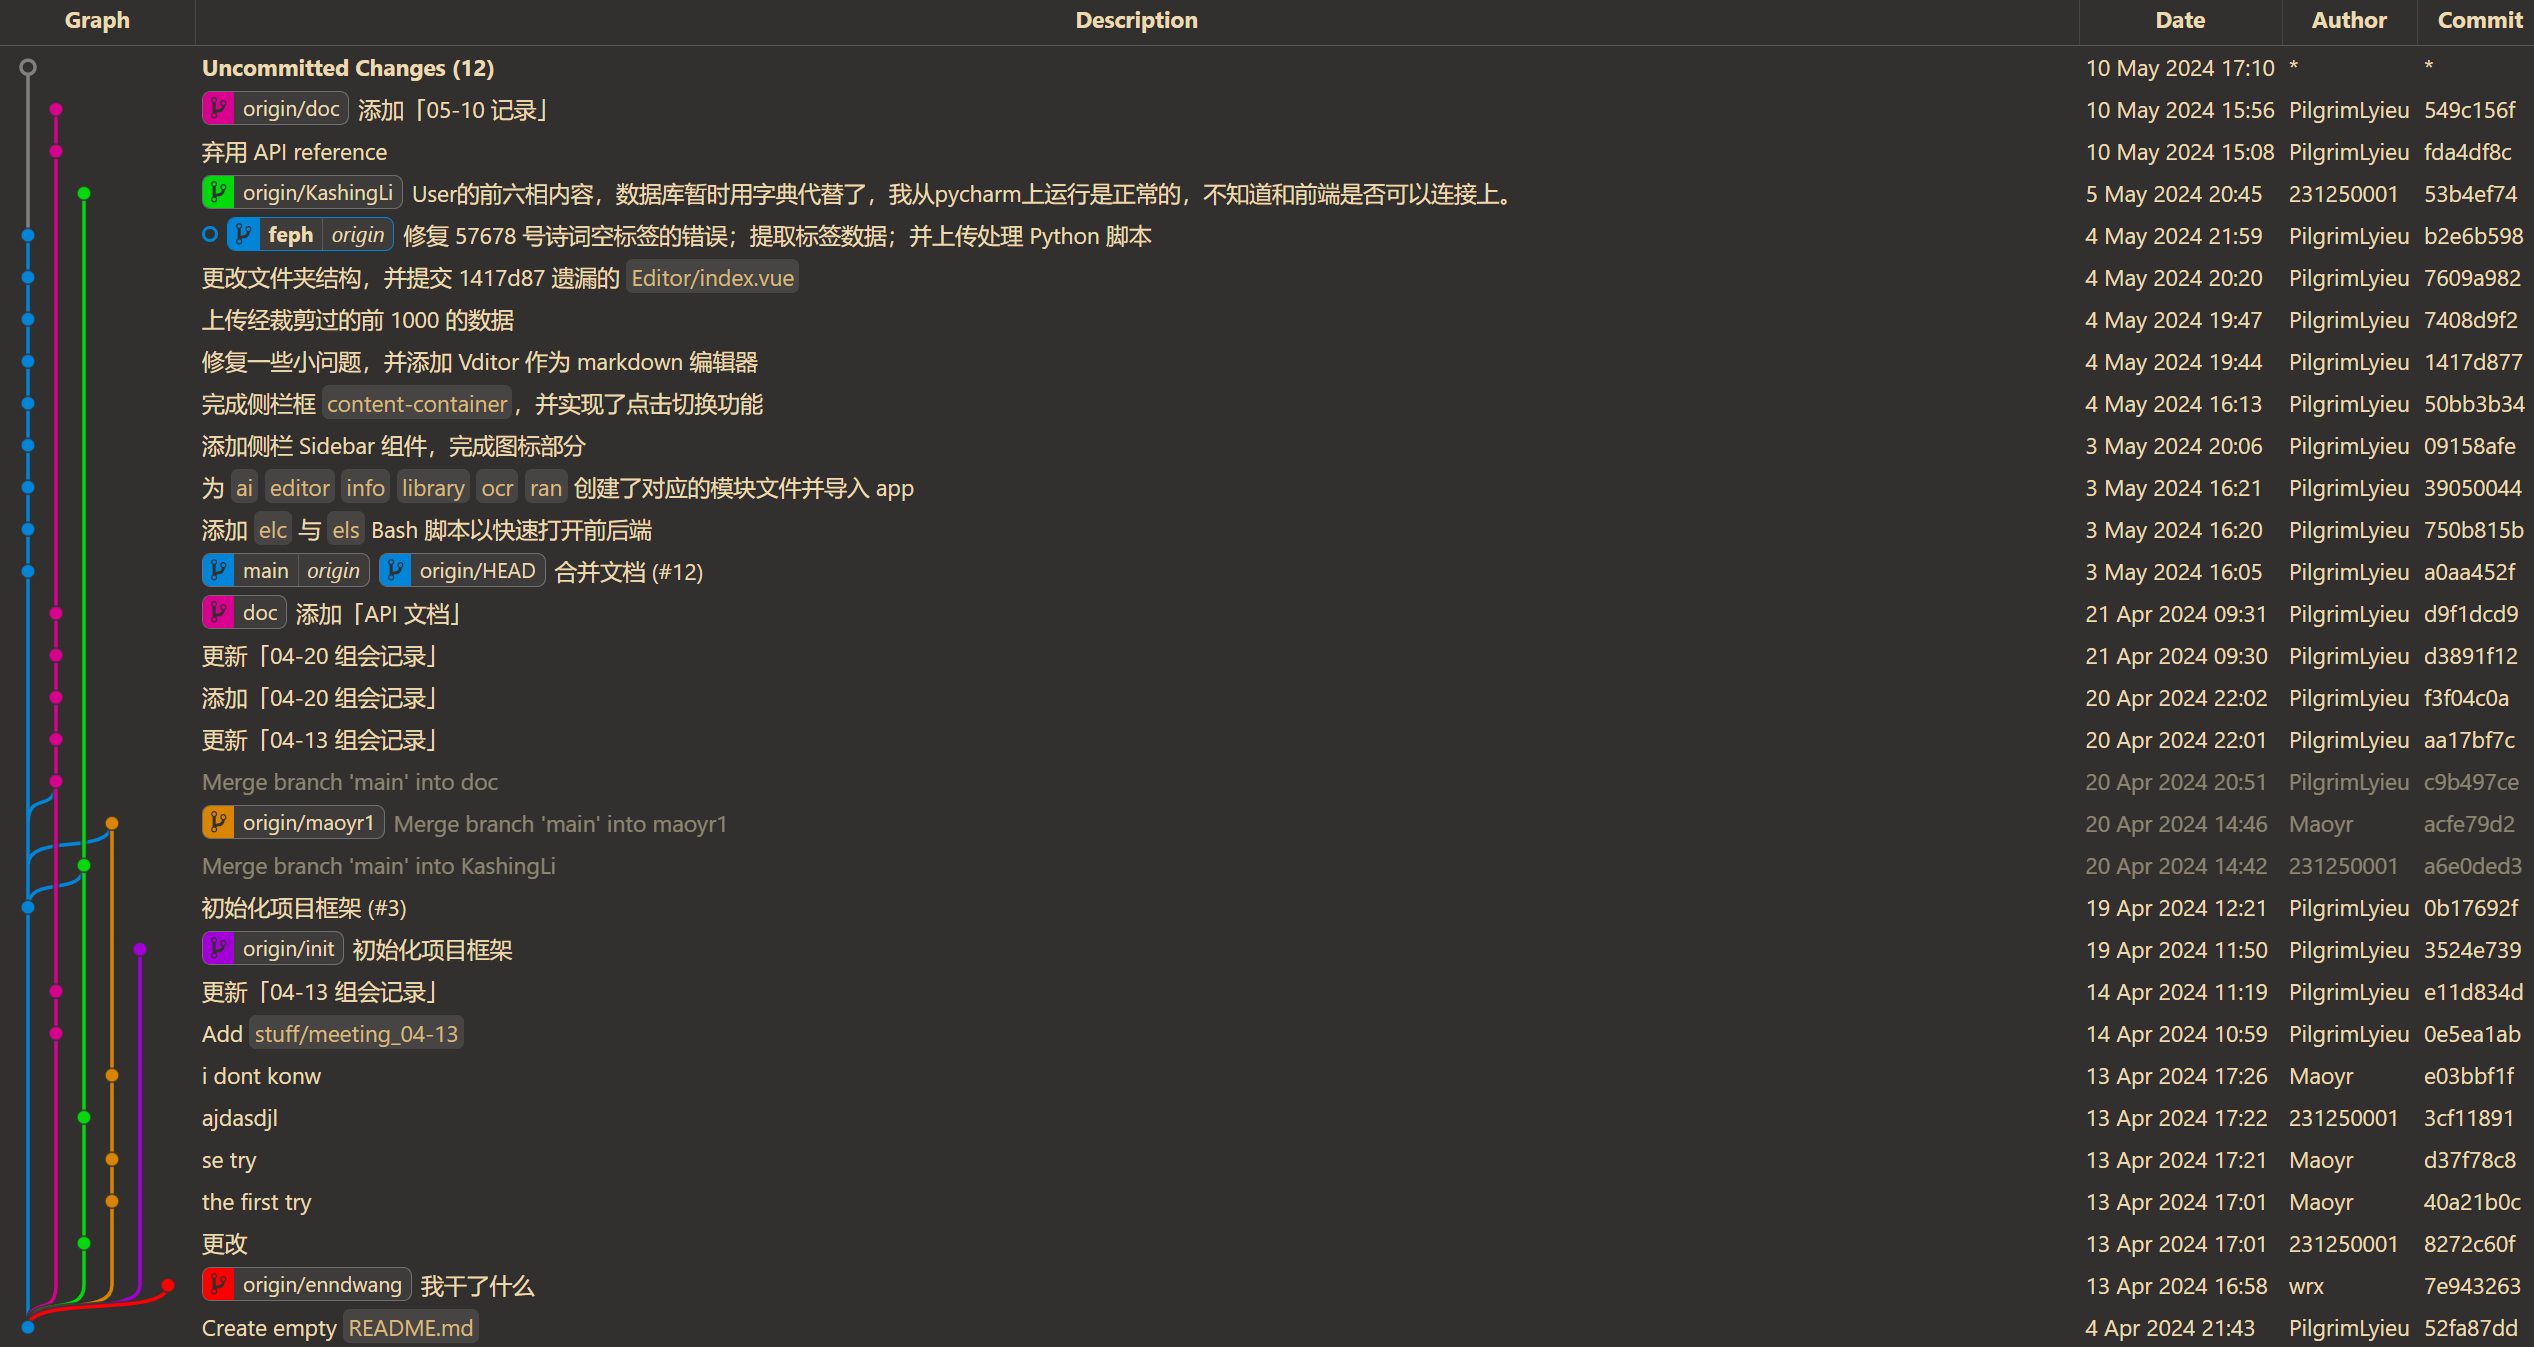
\includegraphics[scale=0.18]{img/commits.png}
\end{figure}

当前的成品也如第一张图所示,目前仅完成了框架部分,接下来还需要对功能栏的每个功能组件进行开发。

\end{document}
